\documentclass[]{beamer}
%\documentclass[handout]{beamer}
%\usetheme[hideothersubsections]{PaloAlto}

\usepackage{amsmath,amssymb,bm,array,graphicx}
\usepackage{multirow, dcolumn}
%\usepackage{movie15}
%\bibliographystyle{jasa}
\graphicspath{{./}{figs/}}
\setbeamercovered{transparent}
\title{Bayesian Adaptive Regression Kernels}
%\author[M. Clyde]{Merlise Clyde}
\date{\today}
\newcommand{\bs}[2]{\begin{frame} \frametitle{#1}
{#2}
\end{frame} }
\usepackage{xcolor}
\definecolor{beamer@blendedblue}{RGB}{86,155,189}
\definecolor{myblue}{RGB}{12,76,138}
\setbeamercolor{structure}{fg=myblue}
\definecolor{Ftitle}{RGB}{12,76,138}
\definecolor{Descitem}{RGB}{238,238,244}
\definecolor{StdTitle}{RGB}{12,76,138}
\definecolor{StdBody}{RGB}{213,24,0}
\definecolor{StdBody}{RGB}{213,24,0}

\definecolor{AlTitle}{RGB}{255, 190, 190}
\definecolor{AlBody}{RGB}{213,24,0}

\definecolor{ExTitle}{RGB}{201, 217, 217}
\definecolor{ExBody}{RGB}{213,24,0}

\setbeamercolor{frametitle}{fg = Ftitle}
\setbeamercolor{title}{fg = Ftitle}
\setbeamercolor{item}{fg = Ftitle}
\setbeamercolor{subitem}{fg = Ftitle}
\setbeamercolor{subsubitem}{fg = Ftitle}
\setbeamercolor{description item}{fg = myblue}
\setbeamercolor{titlelike}{fg=myblue}

%$Id: macros.tex,v 1.2 2006/02/13 14:23:55 rlw Exp rlw $
\newcommand{\Lmea}{{\cal L}} 
\newcommand{\scale}{\bflambda} 
\newcommand{\Scale}{\bfLambda} 
\newcommand{\bfscale}{\bflambda} 
\newcommand{\mean}{\bfchi}
\newcommand{\loc}{\bfchi}
\newcommand{\bfmean}{\bfchi}
\renewcommand{\k}{g}
\newcommand{\Gen}{{\cal G}}
\newcommand{\eps}{\epsilon}

\newcommand{\ind}{\mathrel{\mathop{\sim}\limits^{\mathit{ind}}}}
\newcommand{\iid}{\mathrel{\mathop{\sim}\limits^{\mathit{iid}}}}
\newcommand{\dis}{\mathrel{\mathop{=}\limits^{d}}}
\newcommand{\sgn}{\mathop{\rm sgn}}
\newcommand{\cmp}{h}
\newcommand{\dbdo}{d\beta ~ d\omega}
\newcommand{\real}{{\mathbb{R}}}
\newcommand{\Ber}{\mbox{\rm Ber}}
\newcommand{\GP}{\mbox{\rm GP}}
\newcommand{\SaS}{\text{S$\alpha$S}}
\newcommand{\RA}{{\real \times A}}
\newcommand{\RK}{{\real \times K}}
\newcommand{\RO}{{\real \times \Omega}} 
\newcommand{\RS}{{\bbR \times \LamS}}
  \newcommand{\set}[1]{\left\{#1\right\}}
  \newcommand{\bet}[1]{\left[#1\right]}
  \newcommand{\cet}[1]{\left(#1\right)}
%  \renewcommand{\half}{{\scriptstyle\frac12}}
\newcommand{\subA}{(\eps_1 < \beta \le \eps_2) \times \LamS}
 \newcommand{\uu}{{\big(\scale(x - \loc)\big)}}
 \newcommand{\uuj}{{\big(\scale_j(x-\loc_j)\big)}}
 \newcommand{\bbT}{{\mathbb{T}}}
 \newcommand{\ui}{{[0,1)}}
 \newcommand{\spq}[1]{\left|#1\right|^s_{pq}}
 \newcommand{\spqper}[1]{\left|#1\right|^{s\,*}_{pq}}
 \newcommand{\sspqper}[1]{\left\|#1\right\|^{s\,*}_{pq}}
 \newcommand{\sspq}[1]{\left\|#1\right\|^s_{pq}}    % Besov semi-norm
 \newcommand{\qp}[1]  {\left\|#1\right\|^q_p}         % Hilbert-space norm
 \newcommand{\qper}[1]{\left\|#1\right\|^{*\,q}_p}  % Periodic HS norm
 

\newcommand{\bbW}{{\mathbb{W}}}
\newcommand{\bbB}{{\mathbb{B}}}
\newcommand{\Sob}{{\ensuremath{\bbW^s_2}}}
\newcommand{\Besov}{{\ensuremath{\bbB^s_{pq}}}}
\newcommand{\Besper}{{\ensuremath{\bbB^{s\,*}_{pq}}}}
\newcommand{\Sobx}[1]{{\bbW^{#1}_2}}
\newcommand{\Besovx}[1]{{\bbB^{#1}_2}}
\newcommand{\SN}[1]{\|{#1}\|_\Sob}
% MATH LETTER DEFINITIONS
\newcommand{\Levy}{L{\'e}vy}
\newcommand{\nmathbf}{\bm}
\newcommand{\tabb}[1]{\hspace*{#1\parindent}}
%\newcommand{\G}{{g}}    % Really the same as \GB
\newcommand{\g}{{\phi}} %\newcommand{\g}{{g}}
\newcommand{\GB}{{g}}  
% Roman math Bold face 


\def\bfA{\nmathbf A}
\def\bfB{\nmathbf B}
\def\bfC{\nmathbf C}
\def\bfD{\nmathbf D}
\def\bfE{\nmathbf E}
\def\bfF{\nmathbf F}
\def\bfG{\nmathbf G}
\def\bfH{\nmathbf H}
\def\bfI{\nmathbf I}
\def\bfJ{\nmathbf J}
\def\bfK{\nmathbf K}
\def\bfL{\nmathbf L}
\def\bfM{\nmathbf M}
\def\bfN{\nmathbf N}
\def\bfO{\nmathbf O}
\def\bfP{\nmathbf P}
\def\bfQ{\nmathbf Q}
\def\bfR{\nmathbf R}
\def\bfS{\nmathbf S}
\def\bfT{\nmathbf T}
\def\bfU{\nmathbf U}
\def\bfV{\nmathbf V}
\def\bfW{\nmathbf W}
\def\bfX{\nmathbf X}
\def\bfY{\nmathbf Y}
\def\bfZ{\nmathbf Z}

\def\bfa{\nmathbf a}
\def\bfb{\nmathbf b}
\def\bfc{\nmathbf c}
\def\bfd{\nmathbf d}
\def\bfe{\nmathbf e}
\def\bff{\nmathbf f}
\def\bfg{\nmathbf g}
\def\bfh{\nmathbf h}
\def\bfi{\nmathbf i}
\def\bfj{\nmathbf j}
\def\bfk{\nmathbf k}
\def\bfl{\nmathbf l}
\def\bfm{\nmathbf m}
\def\bfn{\nmathbf n}
\def\bfo{\nmathbf o}
\def\bfp{\nmathbf p}
\def\bfq{\nmathbf q}
\def\bfr{\nmathbf r}
\def\bfs{\nmathbf s}
\def\bft{\nmathbf t}
\def\bfu{\nmathbf u}
\def\bfv{\nmathbf v}
\def\bfw{\nmathbf w}
\def\bfx{\nmathbf x}
\def\bfy{\nmathbf y}
\def\bfz{\nmathbf z}


\def\bfalpha  {\nmathbf \alpha}
\def\bfbeta   {\nmathbf \beta}
\def\bfgamma  {\nmathbf \gamma}
\def\bfdelta  {\nmathbf \delta}
\def\bfepsilon{\nmathbf \epsilon}
\def\bfvareps {\nmathbf \varepsilon}
\def\bfzeta   {\nmathbf \zeta}
\def\bfeta    {\nmathbf \eta}
\def\bftheta  {\nmathbf \theta}
\def\bfiota   {\nmathbf \iota}
\def\bfkappa  {\nmathbf \kappa}
\def\bflambda {\nmathbf \lambda}
\def\bfmu     {\nmathbf \mu}
\def\bfnu     {\nmathbf \nu}
\def\bfxi     {\nmathbf \xi}
\def\bfomicron{\nmathbf \omicron}
\def\bfpi     {\nmathbf \pi}
\def\bfrho    {\nmathbf \rho}
\def\bfsigma  {\nmathbf \sigma}
\def\bftau    {\nmathbf \tau}
\def\bfupsilon{\nmathbf \upsilon}
\def\bfphi    {\nmathbf \phi}
\def\bfpsi    {\nmathbf \psi}
\def\bfchi    {\nmathbf \chi}
\def\bfomega  {\nmathbf \omega}
\newcommand{\nubw}{{\tilde\nu}}  % no longer red!
\def\bfAlpha  {\nmathbf \Alpha}
\def\bfBeta   {\nmathbf \Beta}
\def\bfGamma  {\nmathbf \Gamma}
\def\bfDelta  {\nmathbf \Delta}
\def\bfEpsilon{\nmathbf \Epsilon}
\def\bfZeta   {\nmathbf \Zeta}
\def\bfEta    {\nmathbf \Eta}
\def\bfTheta  {\nmathbf \Theta}
\def\bfIota   {\nmathbf \Iota}
\def\bfKappa  {\nmathbf \Kappa}
\def\bfLambda {\nmathbf \Lambda}
\def\bfMu     {\nmathbf \Mu}
\def\bfNu     {\nmathbf \Nu}
\def\bfXi     {\nmathbf \Xi}
\def\bfOmicron{\nmathbf \Omicron}
\def\bfPi     {\nmathbf \Pi}
\def\bfRho    {\nmathbf \Rho}
\def\bfSigma  {\nmathbf \Sigma}
\def\bfTau    {\nmathbf \Tau}
\def\bfUpsilon{\nmathbf \Upsilon}
\def\bfPhi    {\nmathbf \Phi}
\def\bfPsi    {\nmathbf \Psi}
\def\bfChi    {\nmathbf \Chi}
\def\bfOmega  {\nmathbf \Omega}

% Number math Bold face

\newcommand{\bfzero}{{\nmathbf 0}}
\newcommand{\bfone}{{\nmathbf 1}}

% Estimators

\newcommand{\ttheta}{\tilde{\theta}}
\newcommand{\htheta}{\hat{\theta}}
\newcommand{\tbtheta}{\tilde{\bftheta}}
\newcommand{\hbtheta}{\hat{\bftheta}}
\newcommand{\tomega}{\tilde{\omega}}
\newcommand{\homega}{\hat{\omega}}
\newcommand{\tbomega}{\tilde{\bfomega}}
\newcommand{\hbomega}{\hat{\bfomega}}
\newcommand{\tlambda}{\tilde{\lambda}}
\newcommand{\hlambda}{\hat{\lambda}}
\newcommand{\tblambda}{\tilde{\bflambda}}
\newcommand{\hblambda}{\hat{\bflambda}}


% Calligraphic

\newcommand{\mc}[1]{\ensuremath{\mathcal{#1}}}

\newcommand{\cfA}{\mc{A}}
\newcommand{\cfB}{\mc{B}}
\newcommand{\cfC}{\mc{C}}
\newcommand{\cfD}{\mc{D}}
\newcommand{\cfE}{\mc{E}}
\newcommand{\cfF}{\mc{F}}
\newcommand{\cfG}{\mc{G}}
\newcommand{\cfH}{\mc{H}}
\newcommand{\cfI}{\mc{I}}
\newcommand{\cfJ}{\mc{J}}
\newcommand{\cfK}{\mc{K}}
\newcommand{\cfL}{\mc{L}}
\newcommand{\cfM}{\mc{M}}
\newcommand{\cfN}{\mc{N}}
\newcommand{\cfO}{\mc{O}}
\newcommand{\cfP}{\mc{P}}
\newcommand{\cfQ}{\mc{Q}}
\newcommand{\cfR}{\mc{R}}
\newcommand{\cfS}{\mc{S}}
\newcommand{\cfT}{\mc{T}}
\newcommand{\cfU}{\mc{U}}
\newcommand{\cfV}{\mc{V}}
\newcommand{\cfX}{\mc{X}}
\newcommand{\cfY}{\mc{Y}}
\newcommand{\cfZ}{\mc{Z}}

\newcommand{\bmc}[1]{\ensuremath{\boldsymbol{\mathcal{#1}}}}

\newcommand{\bcfA}{\bmc{A}}
\newcommand{\bcfB}{\bmc{B}}
\newcommand{\bcfC}{\bmc{C}}
\newcommand{\bcfD}{\bmc{D}}
\newcommand{\bcfE}{\bmc{E}}
\newcommand{\bcfF}{\bmc{F}}
\newcommand{\bcfG}{\bmc{G}}
\newcommand{\bcfH}{\bmc{H}}
\newcommand{\bcfI}{\bmc{I}}
\newcommand{\bcfJ}{\bmc{J}}
\newcommand{\bcfK}{\bmc{K}}
\newcommand{\bcfL}{\bmc{L}}
\newcommand{\bcfM}{\bmc{M}}
\newcommand{\bcfN}{\bmc{N}}
\newcommand{\bcfO}{\bmc{O}}
\newcommand{\bcfP}{\bmc{P}}
\newcommand{\bcfQ}{\bmc{Q}}
\newcommand{\bcfR}{\bmc{R}}
\newcommand{\bcfS}{\bmc{S}}
\newcommand{\bcfT}{\bmc{T}}
\newcommand{\bcfU}{\bmc{U}}
\newcommand{\bcfV}{\bmc{V}}
\newcommand{\bcfW}{\bmc{W}}
\newcommand{\bcfX}{\bmc{X}}
\newcommand{\bcfY}{\bmc{Y}}
\newcommand{\bcfZ}{\bmc{Z}}

% Special symbols

\newcommand{\reals}{\mbox{\rm I\kern-.20em R}}
\newcommand{\sreals}{\mbox{\small \rm I\kern-.20em R}}
\newcommand{\LamS}{{\cS^d_+}}

% MATHEMATICAL NOTATION

% Operators

\newcommand{\bg}{\;\bigg\vert\;}
\newcommand{\pr}{\mbox{\rm Pr}}
\newcommand{\D}{\mbox{\rm D}}
\newcommand{\E}{\mbox{\rm E}}
\newcommand{\Mo}{\mbox{\rm Mo}}
\newcommand{\Me}{\mbox{\rm Me}}
\newcommand{\Cov}{\mbox{\rm Cov}}
\newcommand{\Var}{\mbox{\rm Var}}
\newcommand{\Corr}{\mbox{\rm Corr}}
\newcommand{\Q}{\mbox{\rm Q}}

% Distributions
\newcommand{\BeBi}{\mbox{\rm BeBi}}
\newcommand{\Be}{\mbox{\rm Be}}
\newcommand{\Bi}{\mbox{\rm Bi}}
\newcommand{\Br}{\mbox{\rm Br}}
\newcommand{\Ca}{\mbox{\rm Ca}}
\newcommand{\Di}{\mbox{\rm Di}}
\newcommand{\Ex}{\mbox{\rm Ex}}
\newcommand{\Fs}{\mbox{\rm Fs}}
\newcommand{\Ga}{\mbox{\sf G}}
\newcommand{\Ge}{\mbox{\rm Ge}}
\newcommand{\GaGa}{\mbox{\rm GaGa}}
\newcommand{\Hy}{\mbox{\rm Hy}}
\newcommand{\IGa}{\mbox{\rm IGa}}
\newcommand{\IPa}{\mbox{\rm IPa}}
\newcommand{\Lo}{\mbox{\rm Lo}}
\newcommand{\Mu}{\mbox{\rm Mu}}
\newcommand{\N}{\mbox{\rm N}}
\newcommand{\NBi}{\mbox{\rm NBi}}
\newcommand{\NGa}{\mbox{\rm NGa}}
\newcommand{\NWi}{\mbox{\rm NWi}}
\newcommand{\Pa}{\mbox{\rm Pa}}
\newcommand{\Po}{\mbox{\sf P}}
\newcommand{\PoGa}{\mbox{\rm PoGa}}
\newcommand{\Ra}{\mbox{\rm Ra}}
\newcommand{\REx}{\mbox{\rm REx}}
\newcommand{\St}{\mbox{\rm St}}
\newcommand{\Un}{\mbox{\rm Un}}
\newcommand{\Wi}{\mbox{\rm Wi}}

% General Mathematics

\newcommand{\dd}[1]{\,d{#1}}
\newcommand{\barx}{\ensuremath{\bar{x}}}
\newcommand{\comb}[2]{{#1\choose#2}}
\newcommand{\ontop}[2]{{#1\atop#2}}
\newcommand{\h}{{\small\ensuremath{1\over2}}}
\newcommand{\hh}[2]{{\small\ensuremath{#1\over#2}}}

\newcommand{\fn}[1]{\hbox{\textrm{#1}}}
\newcommand{\cred}{\fn{Cr}}
\newcommand\dlim{\mathop{\rm \hbox{$\delta$}lim}}
\newcommand{\goto}{\rightarrow}
\newcommand{\gotoinf}{\rightarrow \infty}

\newcommand{\data}{\ensuremath{\bfx=\{x_1,\ldots,x_n\}}}
\newcommand{\brow}[2]{\ensuremath{\{{#1}_1,\ldots,{#1}_{#2}\}}}
\newcommand{\prow}[2]{\ensuremath{({#1}_1,\ldots,{#1}_{#2})}}

\newcommand{\met}{\thinspace{\rm m}}\newcommand{\km}{\thinspace{\rm km}}
\newcommand{\xbar}{\overline X}%
\newcommand{\xbbar}{\overline{\overline X}}%
\font\ss=cmss12
 \newcommand{\OFP}{(\Omega,\cF,\P)}
 \newcommand{\bbC}{\mathbb{C}}
 \newcommand{\bbF}{\mathbb{F}}
 \newcommand{\bbN}{\mathbb{N}}
 \newcommand{\bbR}{\mathbb{R}}
 \newcommand{\bbX}{\mathbb{X}}
 \newcommand{\bbZ}{\mathbb{Z}}
 \newcommand{\one}[1]{\mathbf{1}_{\{#1\}}}
 \newcommand{\cA}{{\cal A}}
 \newcommand{\cB}{{\cal B}} 
 \newcommand{\cE}{{\cal E}}
 \newcommand{\cF}{{\cal F}}
 \newcommand{\cG}{{\cal G}}
 \newcommand{\cH}{{\cal H}}
 \newcommand{\cM}{{\cal M}}
 \newcommand{\cR}{{\cal R}}
 \newcommand{\cS}{{\cal S}}
 \newcommand{\cT}{{\cal T}}
 \newcommand{\cX}{{\cal X}}
 \newcommand{\cY}{{\cal Y}}
 \newcommand{\cZ}{{\cal Z}}
 \newcommand{\eF}{{\CMcal F}}
 \newcommand{\eG}{{\CMcal G}} 
 \newcommand{\eH}{{\CMcal H}}
 \renewcommand{\P}{{\sf{P}}} 
 \renewcommand{\E}{{\sf{E}}}
 \newcommand{\Ev}{{\sf{Ev}}}%
 \newcommand{\V}{{\sf{V}}} 
 \renewcommand{\Cov}{{\sf{Cov}}}
 %\newcommand{\Be}{\textsf{Be}}
 %\newcommand{\Bi}{\textsf{Bi}}
 %\newcommand{\Ex}{\textsf{Ex}}\newcommand{\Ga}{\textsf{Ga}}
 %\newcommand{\Di}{\textsf{Di}}\newcommand{\Ge}{\textsf{Ge}}
 %\newcommand{\IG}{\textsf{IG}}\newcommand{\Lv}{\textsf{Lv}}
 %\newcommand{\HG}{\textsf{HG}}\newcommand{\MN}{\textsf{MN}}
\newcommand{\NB}{\textsf{NB}}\newcommand{\No}{\textsf{N}}
\newcommand{\LN}{\textsf{LN}}
\newcommand{\Lv}{\mbox{\rm Lv}}
%\newcommand{\Pa}{\textsf{Pa}}
% \newcommand{\Po}{\textsf{Po}}\newcommand{\Un}{\textsf{Un}}
 \newcommand{\argmax}{\textrm{argmax}}
 \renewcommand{\th}{{\ensuremath^{\mbox{\tiny th}}}}
 \newcommand{\nd}{{\ensuremath^{\mbox{\tiny nd}}}}
 \newcommand{\st}{{\ensuremath^{\mbox{\tiny st}}}}
 \newcommand{\ii}{{\ensuremath{\bar{i}}}}% \newcommand{\ii}{{\hat i}}
 \newcommand{\jj}{{\ensuremath{\bar{j}}}}%
 \newcommand{\R}{\texttt{R}}
 \newcommand{\mayeq}{\mathrel{\mathop{=}\limits^?}}
 \newcommand{\pperp}{\mathrel{{\rlap{$~\perp$}\perp\,\,}}}
 \newbox\asbox
 \setbox\asbox=\hbox{\vrule height 15pt depth3.5pt width0pt}
 \def\astrut{\relax\ifmmode\copy\strutbox\else\unhcopy\strutbox\fi}
 \def\Strut{\vrule width0pt height 16pt depth 4pt}%
%\font\tinyss=cmss8 at 8truept % for ^T etc
\newcommand{\tsf}[1]{\textsf{\tiny{#1}}}
\newcommand{\fxa}{\mbox{$f(x\mid\alpha)$}}
\newcommand{\fxt}{\mbox{$f(x\mid\theta)$}}
\newcommand{\fxat}{\mbox{$f(x\mid\alpha,\theta)$}}
\newcommand{\tp}{^{\tsf{T}}}
\newcommand{\as}{\textit{a.s.}}
\newcommand{\ie}{\textit{i.e.{}}}
\newcommand{\etc}{\textit{etc}}
\newcommand{\eg}{\textit{e.g.{}}}%
\newcommand{\half}{{\frac12}}
\newcommand{\Sec}[1]{Section\thinspace(\ref{#1})}
\newcommand{\Thm}[1]{Theorem\thinspace\ref{#1}}
\newcommand{\Cor}[1]{Corollary\thinspace\ref{#1}}
\newcommand{\Eqn}[1]{Equation\thinspace(\ref{#1})}
\newcommand{\Fig}[1]{Figure\thinspace(\ref{#1})}
\newcommand{\Figs}[2]{Figures\thinspace(\ref{#1}) and (\ref{#2})}
\newcommand{\Figab}[2]{Figure\thinspace(\ref{#1}#2)}
\newcommand{\Tab}[1]{Table\thinspace(\ref{#1})}
\newcommand{\jth}{{\ensuremath j^{\mbox{\tiny th}}}}%
\providecommand{\ij}{_{ij}} \newcommand{\ji}[1]{_{ij#1}}%
\newcount\ola \newcount\olb \newcount\olc \newcount\old \newcount\ole
\newcount\och\newcount\level
\newtheorem{cor}{Corollary}
\newtheorem{define}{Definition}
\newtheorem{lem}{Lemma}
\newtheorem{prob}{Problem}
\newtheorem{prop}{Proposition}
\newtheorem{thm}{Theorem}
\def\OL#1{\par\noindent\hangindent=#1\parindent % Outline
  \kern1\hangindent\ignorespaces}%
\def\ol#1{%
    \level=#1
    \ifcase\level
    \ola=0 \olb=0 \olc=0 \old=0 \ole=0\or         % Level 0 (reset)
    \olb=0 \olc=0 \old=0 \ole=0 \advance\ola by 1 % Level 1
    \gdef\olev{\uppercase\expandafter{\romannumeral\ola}} \or
    \olc=0 \old=0 \ole=0 \advance\olb by 1        % Level 2
    \och=64 \advance\och by\olb
    \gdef\olev{\char\och}\or
    \old=0 \ole=0 \advance\olc by 1               % Level 3
    \och=48 \advance\och by\olc
    \gdef\olev{\char\och}\or
    \ole=0 \advance\old by 1                      % Level 4
    \och=96 \advance\och by\old
    \gdef\olev{\char\och}\or
    \advance\ole by 1                             % Level 5
    \gdef\olev{\romannumeral\ole} \or
    \message{Outline depth too deep: #1}\fi
    \ifnum\level>0 \OL\level\llap{\olev.\enspace}\ignorespaces\fi}%
\long\def\comment#1/*#2*/{\endcomment}%
\def\endcomment{\relax}%
%
\makeatletter % Find hours (count1) and minutes (count2) past midnight:
\count1\time \divide\count1 60 \count2=-\count1
\multiply\count2 60 \advance\count2 \time
\edef\now{\two@digits{\the\count1}:\two@digits{\the\count2}}
%\renewcommand\section{\@startsection     % Smaller and sans-serif
%    {section}{1}{\z@}{-3.5ex \@plus -1ex \@minus -.2ex}%
%    {2.3ex \@plus.2ex}{\normalfont\large\bfseries\sffamily}}
%\renewcommand\subsection{\@startsection
%    {subsection}{2}{\z@}{-3.25ex\@plus -1ex \@minus -.2ex}%
%    {1.5ex \@plus .2ex}{\normalfont\large\bfseries\sffamily}}
%\renewcommand\subsubsection{\@startsection
%    {subsubsection}{3}{\z@}{-3.25ex\@plus -1ex \@minus -.2ex}%
%    {1.5ex \@plus .2ex}{\normalfont\normalsize\bfseries\sffamily}}
%\def\@seccntformat#1{\csname the#1\endcsname.\quad} % Add . to sec num's
%\long\def\@makecaption#1#2{%                          Use . not : in cap'ns
%  \vskip\abovecaptionskip
%  \sbox\@tempboxa{#1. #2}%
%  \ifdim \wd\@tempboxa >\hsize
%    #1. #2\par
%  \else
%    \global \@minipagefalse
%    \hb@xt@\hsize{\hfil\box\@tempboxa\hfil}%
%  \fi
%  \vskip\belowcaptionskip}
% BEAMER FIX START
\def\newblock{\beamer@newblock}
% BEAMER FIX END
\makeatother

\def\wbox#1#2#3{{\vcenter{\vbox{\hrule height.#3pt
    \hbox{\vrule width.#3pt height#1pt \kern#2pt \vrule width.#3pt}%
                            \hrule height.#3pt}}}}%
\def\Proof.{\medbreak\noindent{\bf Proof.\enspace}}
\def\qed{{\nobreak\hfill\penalty0\hbox to1truecm{}\nobreak
    \hfill$\wbox634$\par\bigskip}}%



\usepackage{Sweave}
\begin{document}
\Sconcordance{concordance:svm.tex:svm.Rnw:%
1 19 1 1 0 253 1 1 4 3 0 1 2 2 1 3 0 1 2 3 1 2 2 5 1 1 2 1 0 1 1 1 6 13 %
0 1 2 2 1 1 4 1 2 3 1 1 2 1 0 1 2 1 0 2 1 6 0 1 2 5 1 1 2 1 0 1 2 1 0 1 %
1 1 2 4 0 1 2 1 1 1 2 4 0 1 2 182 1 1 2 1 0 3 1 1 2 25 0 3 1 5 0 2 2 36 %
0 1 1 5 0 1 1 4 0 1 3}

\begin{frame}
  \titlepage
\end{frame}




\section{Nonparametric Regression}


\bs{Problem Setting}{
Regression problem
$$ \E[Y \mid \bfx] = f(\bfx), \quad \bfx \in \cfX$$
with unknown function $f(\bfx)$ \pause

Write
$$f(\bfx_i) = \beta_0 + \sum_{j = 1}^n \beta_j k(x_i, x_j)
$$

where  $k(x_i, x_j)$ is a kernel function

\begin{itemize}
  \item Linear Kernel  $$ k(x_i, x_j) = x_i^Tx_j$$
  \item Radial or Gaussian Kernel $$k(x_i, x_j) = \exp(- \frac{\lambda}{2}( (x_i - x_j)^T (x_i - x_j))$$

\end{itemize}

"support vectors"




}

\subsection{Stochastic Expansions}
\bs{Expansions} {

Write function as
 $$f(\bfx_i) = \sum_{j=0}^{J}  \psi(\bfx_i, \bfomega_j)\beta_j$$ in
terms of an (over-complete) dictionary where \pause

  \begin{itemize}
   \item  $\{\beta_j\}$:  unknown coefficients \pause
   \item  $J$: number of terms in expansion (finite or infinite) \pause


 \item $\psi(\bfx,\bfomega_j)$   Dictionary elements from
a ``generator function'' $g$ \pause
  \begin{itemize}
  \item cubic splines
$$   \psi(x_i, \omega_j) =  (x_i - \omega_j)^3_+$$ \pause
  \item multivariate kernels  (Gaussian, Cauchy, Exponential, e.g.)
$$  \psi(\bfx_i, \bfomega_j) =  g(
\bfLambda_j (\bfx - \mean_j)) = \exp\left\{-\frac{1}{2}(\bfx - \mean_j)^T \bfLambda_j (\bfx -
  \mean_j)\right\}$$  \pause
  \item translation and scaling wavelet families  \pause

\item Need not be symmetric!
  \end{itemize}
  \end{itemize}


}


\bs{Kernel Convolution } {
    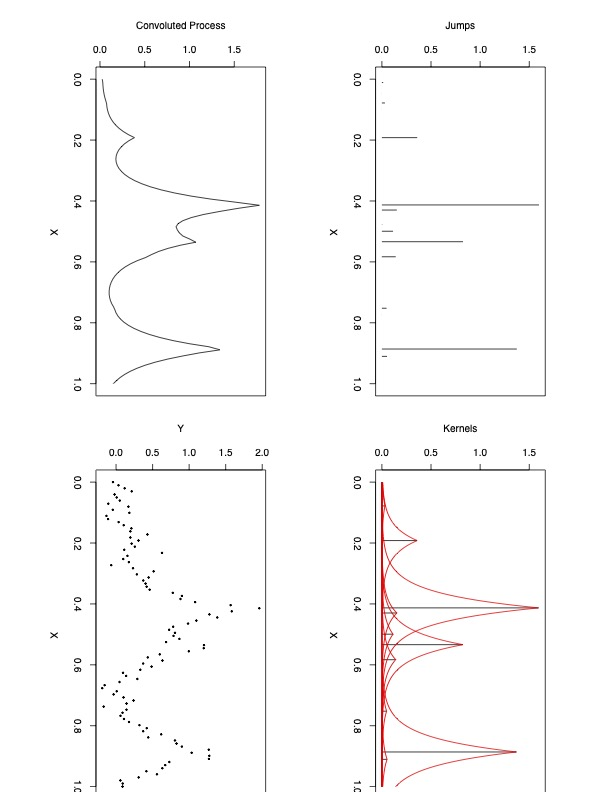
\includegraphics[angle=90,origin=l,totalheight=6.5truecm,
     clip=1, width=10cm]{gammaproc2}

Easy to generate  non-stationarity processes

}







\bs{Bayesian NonParametrics (BNP)}{

Goal $$f(x) = \sum_{j=0}^{J}  \psi(\bfx, \bfomega_j) \beta_j$$
\pause


\pause

\begin{itemize}
\item Poisson prior on $J$  (could be infinite!)
\item[$\Rightarrow$] $J \sim \Po(\nu_+)$,\qquad $\nu_+\equiv
  \nu(\bbR\times\bfOmega) = \iint v(\beta, \bfomega) d \beta \,
  d\bfomega$  \pause
\item[$\Rightarrow$] $\beta_j,\bfomega_j \mid J \iid \pi(\beta, \bfomega)
  \propto \nu(\beta,\bfomega)$. \pause
\end{itemize}

\begin{itemize}
  \item Finite number of ``big'' coefficients $|\beta_j|$ \pause
  \item Possibly infinite number of $\beta \in [-\epsilon, \epsilon]$ \pause
  \item Coefficients $|\beta_j|$ are absolutely summable \pause
  \item Conditions on $\nu$
 \end{itemize}




}


\bs{$\alpha$-Stable L\'evy Measures} {

L\'evy measure: $\nu(\beta, \bfomega) =  c_\alpha |\beta|^{-(\alpha
    +1)}\ \pi(\bfomega) \qquad 0 < \alpha < 2$ \pause

For $\alpha$- Stable $\nu^+(\bbR, \bfOmega) = \infty$ \pause

Fine in theory, but not in practice for MCMC! \pause

\vspace{14pt}
Truncate measure to obtain a finite expansion:
\begin{itemize}
 \item Finite number of support points $\bfomega$ with $\beta$ in
   $[-\epsilon, \epsilon]^c$  \pause
\item Fix $\epsilon$  (for given prior approximation error) \pause
\item Use approximate L\'evy  measure
$\nu_{\epsilon}(\beta, \bfomega) \equiv \nu(\beta,
\bfomega)\bfone(|\beta| > \epsilon) $ \pause
\item[$\Rightarrow$] $J \sim \Po(\nu_{\epsilon}^+)$ where
  $\nu^+_{\epsilon} = \nu([-\epsilon, \epsilon]^c, \bfOmega)$ \pause
\item[$\Rightarrow$]  $\beta_j, \bfomega_j \iid \pi(d\beta, d\bfomega) \equiv
  \nu_\epsilon(d\beta , d \bfomega)/\nu^+_{\epsilon}$ ($\beta_j$
  distributed as Pareto)

\end{itemize}
}


\bs{Truncated Cauchy Process} {
\centerline{Restriction  $|\beta| > \epsilon$}

%\psfrag{x}{\small{$\beta$}}
\centerline{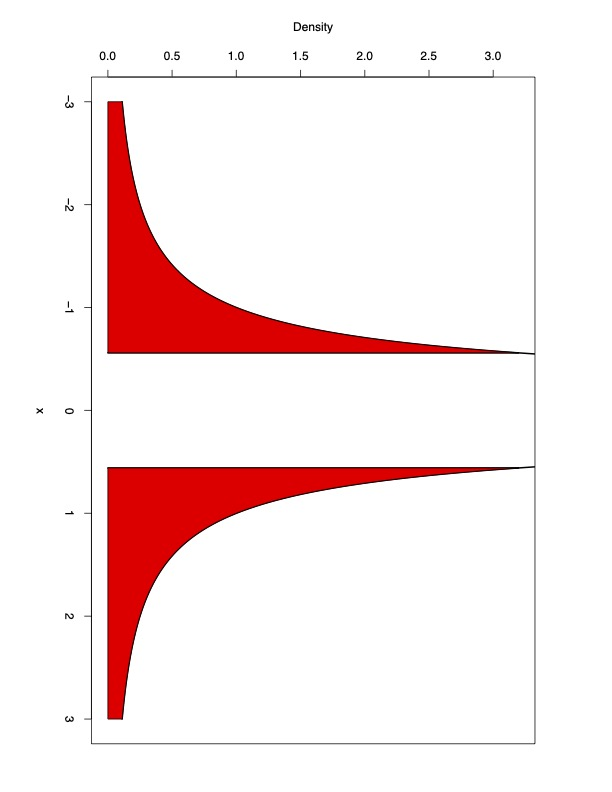
\includegraphics[width=2.5in,angle=90]{cauchy1}}
}


\bs{Contours of Log Prior (in $\bbR^2$) -- Penalties} {
\begin{tabular}{ccc}
Normal  & DE  & Cauchy \\
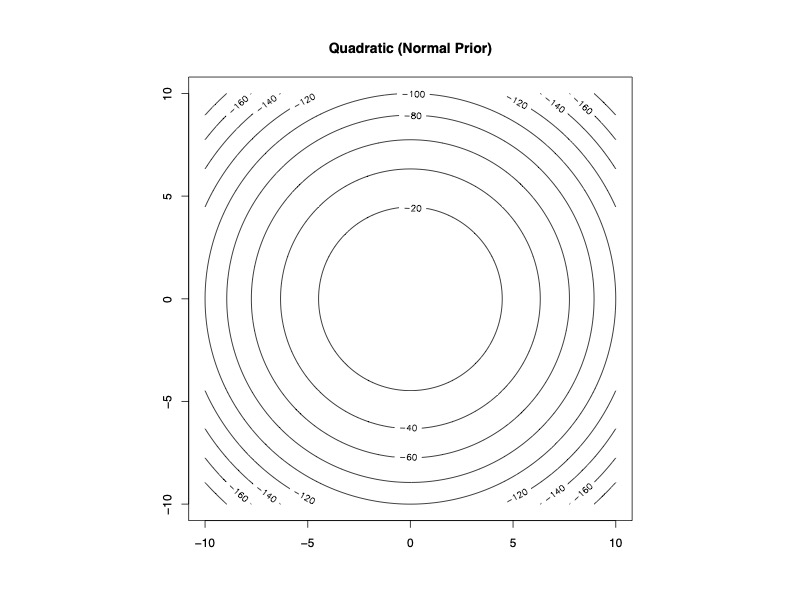
\includegraphics[angle=90,width=1.25in]{L2} &
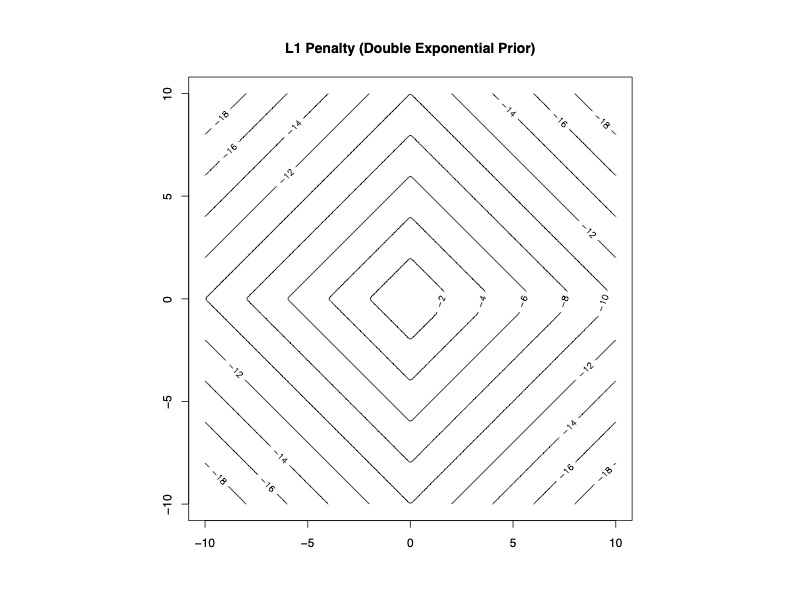
\includegraphics[angle=90,width=1.25in]{L1} &
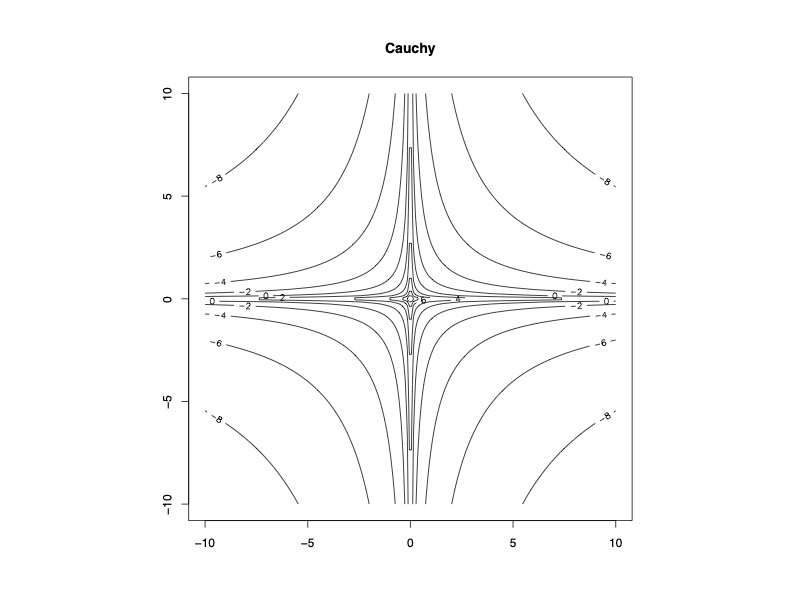
\includegraphics[angle=90,width=1.25in]{cauchy}
\end{tabular}

\vspace{.25in}
Penalized Likelihood:
$$-\frac{1}{2 \sigma^2} \sum_i\left(Y_i - f(\bfx_i)\right)^2  - (\alpha +
1) \sum_j
\log(|\beta_j|)  - \nu^+_{\epsilon} \ldots $$

}





\bs{Higher Dimensional $\cfX$} {

MCMC is (currently) too slow in higher dimensional space to allow \pause
\begin{itemize}
\item $\bfchi$ to be completely arbitrary; restrict support to
  observed $\{\bfx_i\}$ like in SVM \pause
\item use diagonal $\bfLambda$
\end{itemize}
Kernels take form:
\begin{eqnarray*}
\psi(\bfx, \bfomega_j) & = & \prod_d \exp\{ -\frac{1}{2} \lambda_d (x_d - \chi_{d})^2
\} \\
f(\bfx) & =  & \sum_j \psi(\bfx, \bfomega_j) \beta_j
\end{eqnarray*}
}


\bs{Approximate L\'evy Prior II} {
Continuous Approximation Student $t(\alpha, 0, \epsilon)$ approximation:

$$\nu_\epsilon(d\beta, d \bfomega) = c_\alpha (\beta^2 + \alpha
\epsilon^2)^{-(\alpha + 1)/2} d\beta \ \gamma(d \bfomega) $$

\pause

Based on the following hierarchical prior
\begin{eqnarray*}
  \beta_j \mid \phi_j & \ind & \No(0,  \varphi_j^{-1}) \\
  \phi_j    & \ind & \Ga\left(\frac{\alpha}{2}, \frac{\alpha \epsilon^2}{2}\right) \\
   J & \sim & \Po(\nu^+_\epsilon)
\end{eqnarray*}

where $\nu^+_\epsilon = \nu_\epsilon(\bbR, \bfOmega) = \frac{\alpha ^{1
    - \alpha/2} \Gamma(\alpha)\Gamma(\alpha/2)}{\epsilon^\alpha
  \pi^{1/2} \Gamma(\frac{\alpha +1}{2})} \sin(\frac{\pi \alpha} {2}) \gamma(\bfOmega)$

Key:  need to have variance of coefficients decrease as $J$ increases
}

\bs{Limiting Case} {
  \begin{eqnarray*}
    \beta_j   \mid  \varphi_j & \ind &\N(0, 1/\varphi_j) \\
      \varphi_j & \iid & \Ga(\alpha/2, "0")
  \end{eqnarray*}
\pause

Notes:
  \begin{itemize}
\item Require $0 < \alpha < 2$  Additional restrictions  on $\omega$  \pause
\item  Cauchy process corresponds to $\alpha = 1$ \pause
\item  Tipping's ``Relevance Vector Machine'' corresponds to $\alpha =
  0$  (improper posterior!) \pause
\item Provides an extension of {\bf{Generalized Ridge Priors}}
      to infinite dimensional case \pause
\item Infinite dimensional analog of Cauchy priors
 \end{itemize}
}

\bs{Further Simplification in Case with $\alpha = 1$} {
  \begin{itemize}
  \item Poisson number of points $J_\eps\sim \Po\big(
    \nu_\eps^+(\alpha, \gamma) \big)$ with $\nu_\eps^+(\alpha, \gamma)
  = \frac{\gamma \alpha^{1-\alpha/2}}{2^{1 - \alpha}\eps^\alpha}
  \frac{\Gamma(\alpha/2)}{\Gamma(1-\alpha/2)}$ \pause
  \item Given $J$, $[ n_1 : n_n] \sim  MN(J, 1/(n+1))$ points
    supported at each kernel located at $\bfx_j$  \pause
  \end{itemize}
The regression mean function can be rewritten as
\[
  f(\bfx) = \sum_{i=0}^n \tilde{\beta}_i \psi(\bfx, \bfomega_i), \quad
  \tilde{\beta}_i = \sum_{\{j \, \mid \bfchi_j = \bfx_i\}} \beta_j.
\]
\pause
In particular, if $\alpha = 1$, not only the Cauchy process is infinitely
divisible, the approximated Cauchy prior distributions on the regression
coefficients are also infinitely divisible:

$$
  \tilde{\beta}_i  \ind
  \No(0, n_i^2 \tilde{\varphi}_i^{-1}), \qquad
  \tilde{\varphi}_i \iid \Ga( 1/2, \eps^2/2)
$$
\pause
At most $n$ non-zero coefficients!
}

\begin{frame}[fragile] \frametitle{BARK: Bayesian Additive Regression Kernels }
\begin{Schunk}
\begin{Sinput}
> #library(devtools)
> #suppressMessages(install_github("merliseclyde/bark"))
> library(bark)
> set.seed(42)
> n = 500
> circle2 = as.data.frame(sim_circle(n, dim = 2))
\end{Sinput}
\end{Schunk}

\end{frame}

\begin{frame}[fragile] \frametitle{Circle}
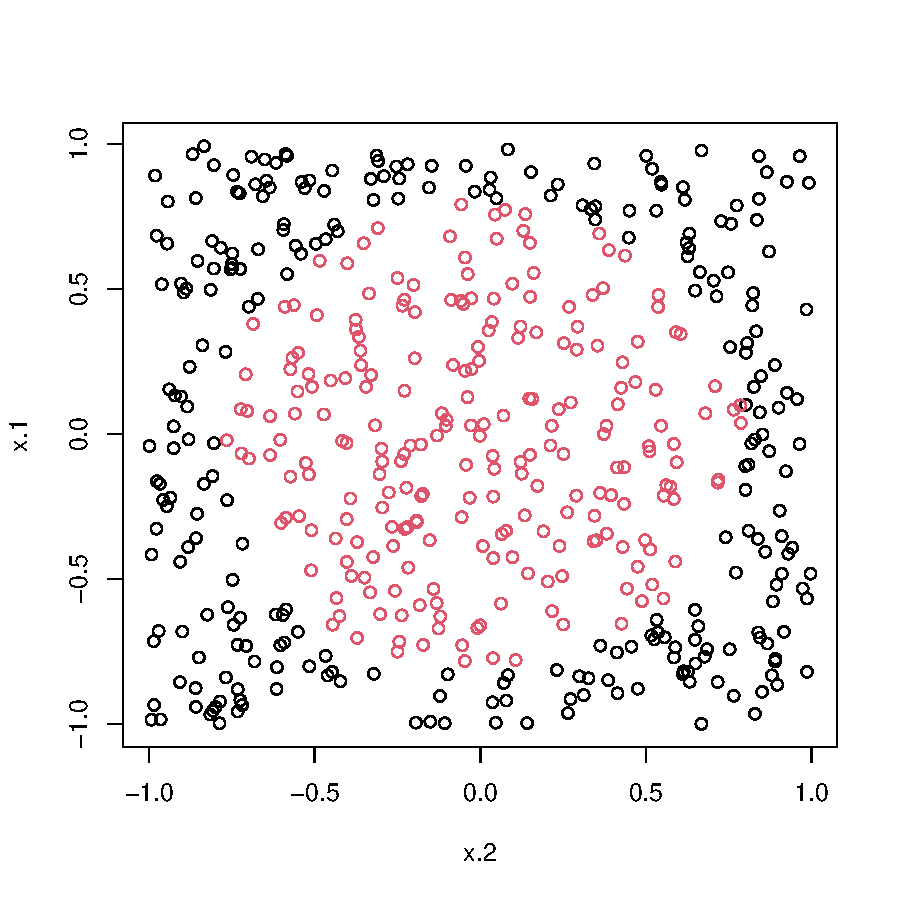
\includegraphics{svm-r}

\end{frame}


\begin{frame}[fragile] \frametitle{Circle Example}

\begin{Schunk}
\begin{Sinput}
> set.seed(42)
> train = sample(1:n, size = floor(n/2), rep=FALSE)
> circle2.bark = bark(as.matrix(circle2[train, 1:2]),
+                     circle2[train, 3],
+                     x.test = as.matrix(circle2[-train, 1:2]),
+                     classification = TRUE,
+                     printevery = 10000,
+                     type="se")
\end{Sinput}
\begin{Soutput}
[1] "Starting BARK-se for this classification problem"
[1] "burning iteration 10000, J=5, max(nj)=2"
[1] "posterior mcmc iteration 10000, J=4, max(nj)=1"
\end{Soutput}
\end{Schunk}
\end{frame}

\begin{frame}[fragile] \frametitle{Missclassification}
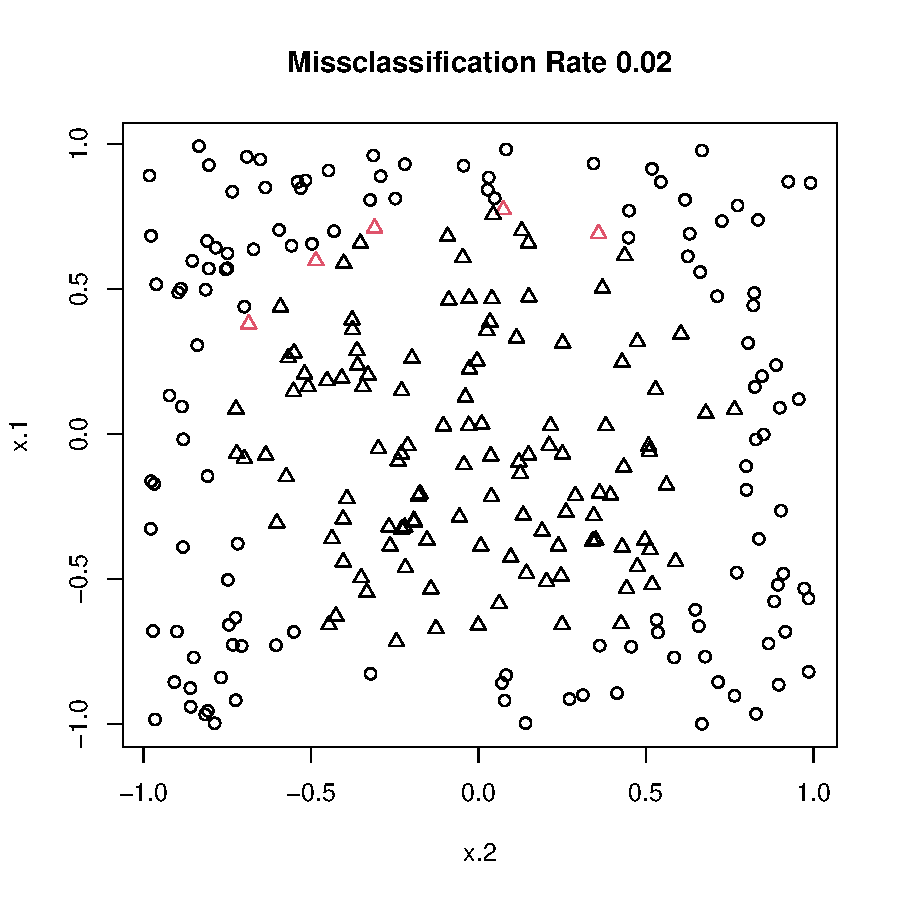
\includegraphics{svm-004}

\end{frame}

\begin{frame}[fragile] \frametitle{SVM}
\begin{Schunk}
\begin{Sinput}
> library(e1071)
> circle2.svm = svm(y ~ x.1 + x.2, data=circle2[train,],
+                   type="C")
> pred.svm = predict(circle2.svm, circle2[-train,])
> mean(pred.svm != circle2[-train, "y"])
\end{Sinput}
\begin{Soutput}
[1] 0.048
\end{Soutput}
\end{Schunk}

\end{frame}



\begin{frame}[fragile] \frametitle{BART}
\begin{Schunk}
\begin{Sinput}
> suppressMessages(library(BART))
> circle.bart = pbart(x.train = circle2[train, 1:2],
+                     y.train = circle2[train, "y"])
> pred.bart = predict(circle.bart, circle2[-train, 1:2])
> mean((pred.bart$prob.test.mean > .5) != 
+        circle2[-train, "y"])
\end{Sinput}
\end{Schunk}


\begin{Schunk}
\begin{Soutput}
[1] 0.036
\end{Soutput}
\end{Schunk}


\end{frame}


\bs{Feature Selection in Kernel} {
\begin{itemize}
\item Product structure allows interactions between variables  \pause
\item Many input variables may be irrelevant \pause
\item Feature selection; if $\lambda_d = 0$ variable $x_d$ is removed
  from all kernels \pause
\item Allow point mass on $\lambda_h = 0$ with probability $p_\lambda
  \sim B(a,b)$  (in practice have used $a = b = 1$ \pause
\end{itemize}

Consider 3 Scenarios

\begin{itemize}
\item $D$ Different $\lambda-D$ parameters in each dimension \pause
\item $S + D$ Different $\lambda_d$ parameters $+$ Selection \pause
\item $S + E$ Selection $+$ Equal for Remaining $\lambda_d = \lambda$
\end{itemize}

}

\section{Examples}

\bs{Regression Out of Sample Prediction} {
Average Relative MSE to best procedure
\small{
  \begin{tabular}[ht]{|l|c|c|c|c|c|}
%  \begin{tabular}[ht]{|l|r|r|c|c|c|c|c|c|}
    \hline
  \multirow{2}{*}{Data Sets} &
%  \multirow{2}{*}{n} &
%  \multirow{2}{*}{p} &
  \multicolumn{3}{c|}{BARK} &
  \multirow{2}{*}{SVM}&
  \multirow{2}{*}{BART} \\
% \cline{4-7}
  \cline{2-4}
% &&& equal & diff
  &  D
  & S $+$ E & S $+$ D && \\
    \hline
  Friedman1       %& 200 & 4
  & 1.22 & 2.26 & 1.93 & 5.36 & 1.97 \\
  Friedman2       %& 200 & 4
  & 1.07 & 1.09 & 1.04 & 4.36 & 3.64 \\
  Friedman3       %& 200 & 4
  & 1.46 & 2.30 & 1.44 & 2.70 & 1.00 \\
  Boston Housing  %& 506 & 13
  & 1.09 & 1.23 & 1.20 & 1.56 & 1.01 \\
  Body Fat        %& 252 & 14
  & 1.81 & 1.01 & 2.19 & 4.04 & 1.68 \\
  Basketball      %& 96  & 4
  & 1.01 & 1.01 & 1.02 & 1.16 & 1.10 \\\hline
  \end{tabular}
}

D: dimension specific scale $\lambda_d$

E: equal scales $\lambda_d = \lambda \, \forall \, d$

S: selection $\lambda_d = 0$ with probability $\rho$

}

%\subsection{Regression}

\bs{Feature Selection in Boston Housing Data} {

Posterior Distribution of $\lambda_d$

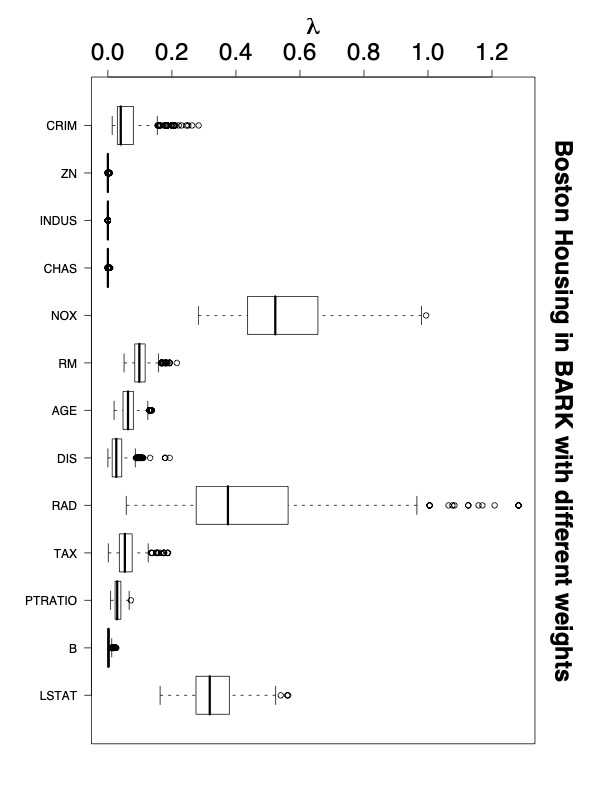
\includegraphics[height=3.5in,angle=90]{bhlambdabox}

}
%\subsection{Classification Examples}
\bs{Classification Examples} {

  \centering
  \begin{tabular}{cccc}
    Name            & $d$ & data type  & $n$ (train/test) \\ \hline
    Circle          &   2 & simulation & 200/1000 \\
    Circle (3 null) &   5 & simulation & 200/1000 \\
    Circle (18 null)&  20 & simulation & 200/1000 \\
    Swiss Bank Notes      &   6 & real data  & 200  $(5\,cv)$ \\
    Breast Cancer   &  30 & real data  & 569 $(5\,cv)$ \\
    Ionosphere      &  33 & real data  & 351 $(5\,cv)$
  \end{tabular}


  \begin{itemize}
  \item Add latent Gaussian $Z_i$ for probit regression \\(as in Albert
  \& Chib)
 \item Same model as before conditional on $\bfZ$
 \item Advantage:  Draw $\bfbeta$ in a block from full conditional
\item Can extend to Logistic
  \end{itemize}

}

\bs{Predictive Error Rate for Classification} {
\small{
 \begin{tabular}[ht]{|l|r|r|r|
%      D{.}{.}{2.3}|D{.}{.}{1.3}|
%      D{.}{.}{4.6}|D{.}{.}{4.4}|
      r|r|}
    \hline
  \multirow{2}{*}{Data Sets} &
%  \multirow{2}*{n} &
%  \multirow{2}*{p} &
  \multicolumn{3}{c|}{BARK} &
  \multirow{2}*{SVM}&
  \multirow{2}*{BART} \\
% \cline{4-7}
  \cline{2-4}
% &&& \multicolumn{1}{c|}{E}
  & \multicolumn{1}{c|}{D}
  & \multicolumn{1}{c|}{S $+$ E}
  & \multicolumn{1}{c|}{S $+$ D} && \\
    \hline
    Circle 2      %&200&  2
     & 4.91\% & 1.88\% & 1.93\% & 5.03\% & 3.97\% \\
    Circle 5      %&200&  5
     & 4.70\% & 1.47\% & 1.65\% & 10.99\% & 6.51\% \\
    Circle 20     %&200& 20
     & 4.84\% & 2.09\% & 3.69\% & 44.10\% & 15.10\% \\
    Bank          %&200& 6
     & 1.25\% & 0.55\% & 0.88\% & 1.12\% & 0.50\% \\
    BC          %&569& 30
     & 4.02\% & 2.49\% & 6.09\% & 2.70\% & 3.36\% \\
    Ionosphere    %&351& 33
     & 8.59\% & 5.78\% &10.87\% & 5.17\% & 7.34\%\\ \hline
  \end{tabular}

D: dimension specific scale $\lambda_d$

E: equal scales $\lambda_d = \lambda \forall d$

S: selection $\lambda_d = 0$ with probability $\rho$
}
}



\section{Summary}

\bs{Needs \& Limitations}{

  \begin{itemize}
  \item NP Bayes of many flavors often does better than frequentist methods
(BARK, BART, Treed GP, more) \pause
\item Hyper-parameter specification - theory \& computational
  approximation \pause
\item need faster code for BARK that is easier for users (BART \& TGP are
  great!)   ({\tt library(bark)} or github \pause
\item Can these models be added to JAGS, STAN, etc instead of
  stand-alone R packages \pause
\item With availability of code what are caveats for users?

  \end{itemize}
}

\bs{Summary} {
L\'evy Random Field Priors \& LARK models:
  \begin{itemize}
  \item Provide limit of finite dimensional priors (GRP \& SVSS) to infinite
  dimensional setting \pause
  \item Adaptive bandwidth for kernel regression \pause
  \item Allow flexible generating functions \pause
  \item Provide sparser representations compared to SVM \& RVM, with
    coherent Bayesian interpretation \pause
  \item Incorporation of  prior knowledge if available \pause
  \item Relax assumptions of equally spaced data and Gaussian likelihood \pause
  \item Hierarchical Extensions \pause
  \item Formulation allows one to define stochastic processes on
    arbitrary spaces (spheres, manifolds)
\end{itemize}
}

\end{document}

\begin{Schunk}
\begin{Sinput}
> n = 200
> t = matrix(sort(runif(n, -10, 10)))
> mu = 1/(1 + exp(-t))
> y = rnorm(n,mu, sd=.1)
> bk = bark(t, y, t, class=FALSE)
\end{Sinput}
\begin{Soutput}
[1] "Starting BARK-se for this regression problem"
[1] "burning iteration 1000, J=12, max(nj)=1"
[1] "burning iteration 2000, J=13, max(nj)=2"
[1] "burning iteration 3000, J=13, max(nj)=2"
[1] "burning iteration 4000, J=7, max(nj)=1"
[1] "burning iteration 5000, J=9, max(nj)=1"
[1] "burning iteration 6000, J=12, max(nj)=1"
[1] "burning iteration 7000, J=8, max(nj)=1"
[1] "burning iteration 8000, J=6, max(nj)=1"
[1] "burning iteration 9000, J=14, max(nj)=2"
[1] "burning iteration 10000, J=11, max(nj)=1"
[1] "posterior mcmc iteration 1000, J=17, max(nj)=1"
[1] "posterior mcmc iteration 2000, J=10, max(nj)=1"
[1] "posterior mcmc iteration 3000, J=13, max(nj)=1"
[1] "posterior mcmc iteration 4000, J=12, max(nj)=1"
[1] "posterior mcmc iteration 5000, J=13, max(nj)=2"
[1] "posterior mcmc iteration 6000, J=14, max(nj)=1"
[1] "posterior mcmc iteration 7000, J=11, max(nj)=1"
[1] "posterior mcmc iteration 8000, J=8, max(nj)=1"
[1] "posterior mcmc iteration 9000, J=11, max(nj)=1"
[1] "posterior mcmc iteration 10000, J=10, max(nj)=1"
\end{Soutput}
\begin{Sinput}
> plot(t, y)
> lines(t, bk$yhat.test.mean, col=2, lty=1)
> mean((mu - bk$yhat.test.mean)^2)
\end{Sinput}
\begin{Soutput}
[1] 0.0007400087
\end{Soutput}
\begin{Sinput}
> suppressMessages(library(BART))
> out.bart = wbart(x.train=t,
+                  y.train = y)
\end{Sinput}
\begin{Soutput}
*****Into main of wbart
*****Data:
data:n,p,np: 200, 1, 0
y1,yn: -0.317372, 0.455214
x1,x[n*p]: -9.974335, 9.979124
*****Number of Trees: 200
*****Number of Cut Points: 100 ... 100
*****burn and ndpost: 100, 1000
*****Prior:beta,alpha,tau,nu,lambda: 2.000000,0.950000,0.025382,3.000000,0.007051
*****sigma: 0.190257
*****w (weights): 1.000000 ... 1.000000
*****Dirichlet:sparse,theta,omega,a,b,rho,augment: 0,0,1,0.5,1,1,0
*****nkeeptrain,nkeeptest,nkeeptestme,nkeeptreedraws: 1000,1000,1000,1000
*****printevery: 100
*****skiptr,skipte,skipteme,skiptreedraws: 1,1,1,1

MCMC
done 0 (out of 1100)
done 100 (out of 1100)
done 200 (out of 1100)
done 300 (out of 1100)
done 400 (out of 1100)
done 500 (out of 1100)
done 600 (out of 1100)
done 700 (out of 1100)
done 800 (out of 1100)
done 900 (out of 1100)
done 1000 (out of 1100)
time: 2s
check counts
trcnt,tecnt,temecnt,treedrawscnt: 1000,0,0,1000
\end{Soutput}
\begin{Sinput}
> mean((out.bart$yhat.train.mean -mu)^2)
\end{Sinput}
\begin{Soutput}
[1] 0.001063777
\end{Soutput}
\begin{Sinput}
> lines(t, out.bart$yhat.train.mean)
> 
\end{Sinput}
\end{Schunk}

